\documentclass[11pt]{article}
\usepackage[margin=1in]{geometry}
\usepackage{graphicx}
\usepackage{float}

\setlength{\parindent}{0pt}
\setlength{\parskip}{6pt}

\title{\vspace{-1.5cm}A Simpler Model Confirms the Wildfire Effect}
\author{}
\date{}

\begin{document}
\maketitle
\vspace{-1.2cm}

\section*{The result}
A \textbf{simpler} approach --- one model trained on \emph{all} the data (wildfire +
clean), compared against a clean-only model --- gives \textbf{the same answer} as the
two-model method: wildfire raises CCN by about \textbf{16\%} during wildfire periods
(Figure~\ref{fig:money}). It recovers this with \textbf{no special handling}, and
giving the wildfire data extra weight \textbf{did not change the answer}
(Figure~\ref{fig:agree}). The all-data model is also somewhat better calibrated than
the wildfire-only model, since it trains on more data.

\begin{figure}[H]
\centering
\begin{minipage}{0.32\textwidth}\centering
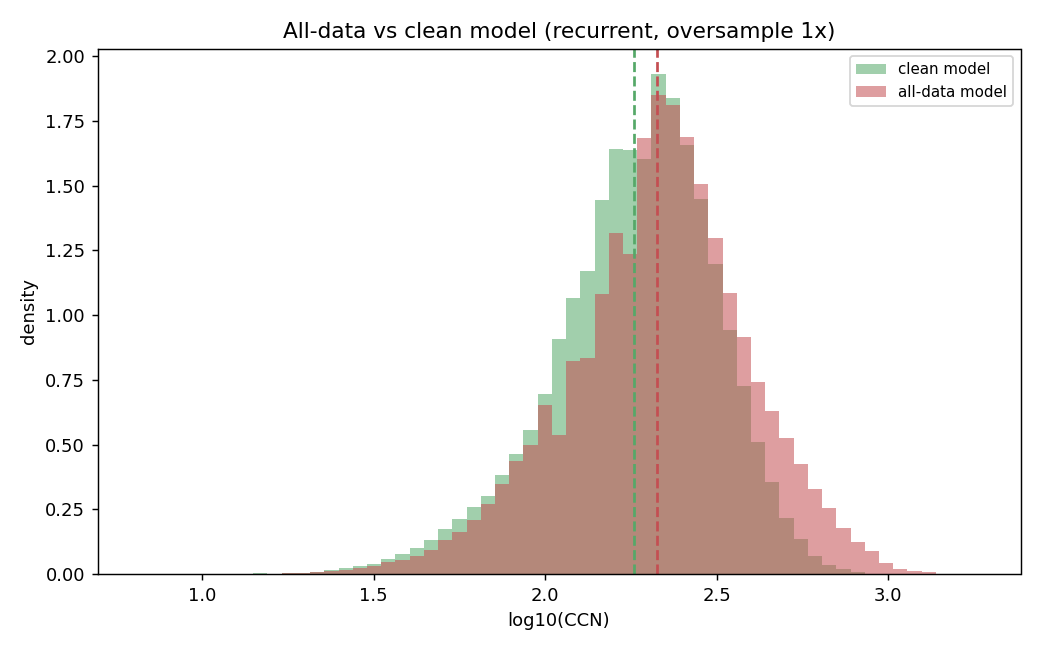
\includegraphics[width=\linewidth]{money_recurrent_os1x.png}\\ \small recurrent
\end{minipage}\hfill
\begin{minipage}{0.32\textwidth}\centering
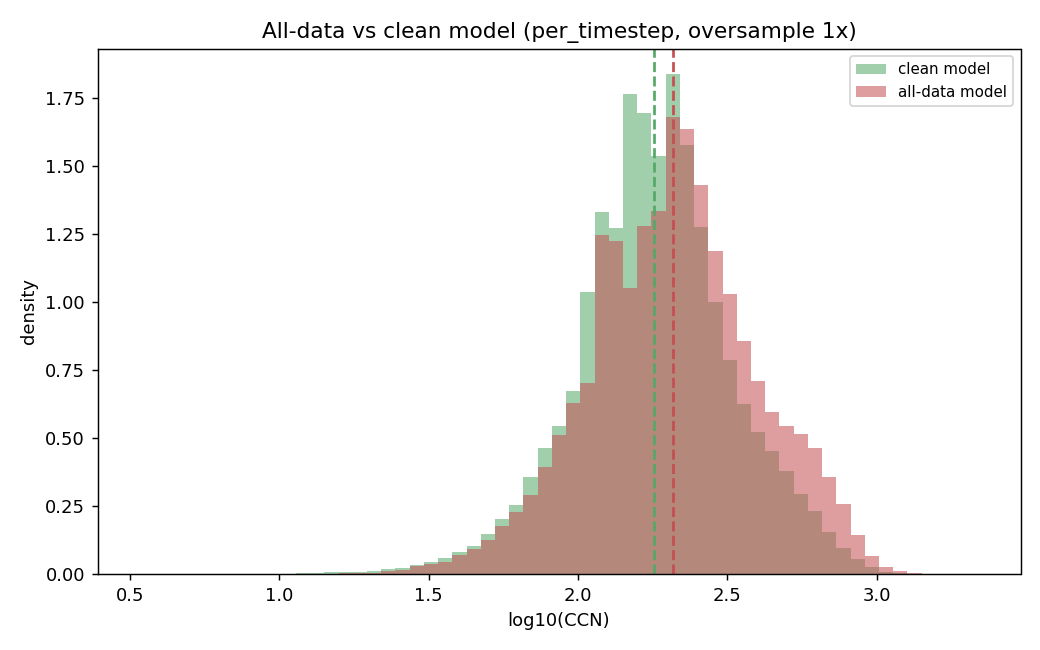
\includegraphics[width=\linewidth]{money_per_timestep_os1x.png}\\ \small per-timestep
\end{minipage}\hfill
\begin{minipage}{0.32\textwidth}\centering
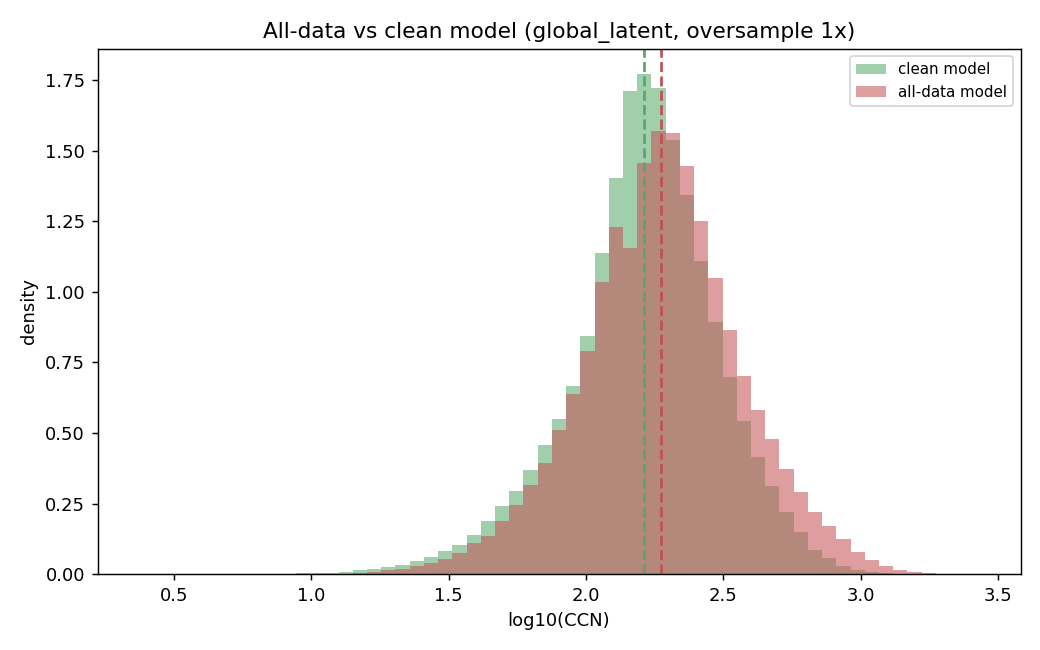
\includegraphics[width=\linewidth]{money_global_latent_os1x.png}\\ \small global-latent
\end{minipage}
\caption{The all-data model (red) vs.\ the clean model (green) at wildfire-period
weather, for all three model types (no oversampling). In every case the all-data
model already sits at higher CCN --- the wildfire effect is present, not washed out.}
\label{fig:money}
\end{figure}

\section*{How the plots were made}
Exactly as in the two-model report, both models are run \emph{at the same weather}:
the weather from the \textbf{held-out wildfire periods}. The \textbf{red} curve is the
\emph{all-data} model's predicted CCN for that weather; the \textbf{green} curve is
the \emph{clean} model's prediction for the same weather (what CCN would have been
without wildfire). Both use the same wildfire-period weather as input; only the model
differs.

\begin{figure}[H]
\centering
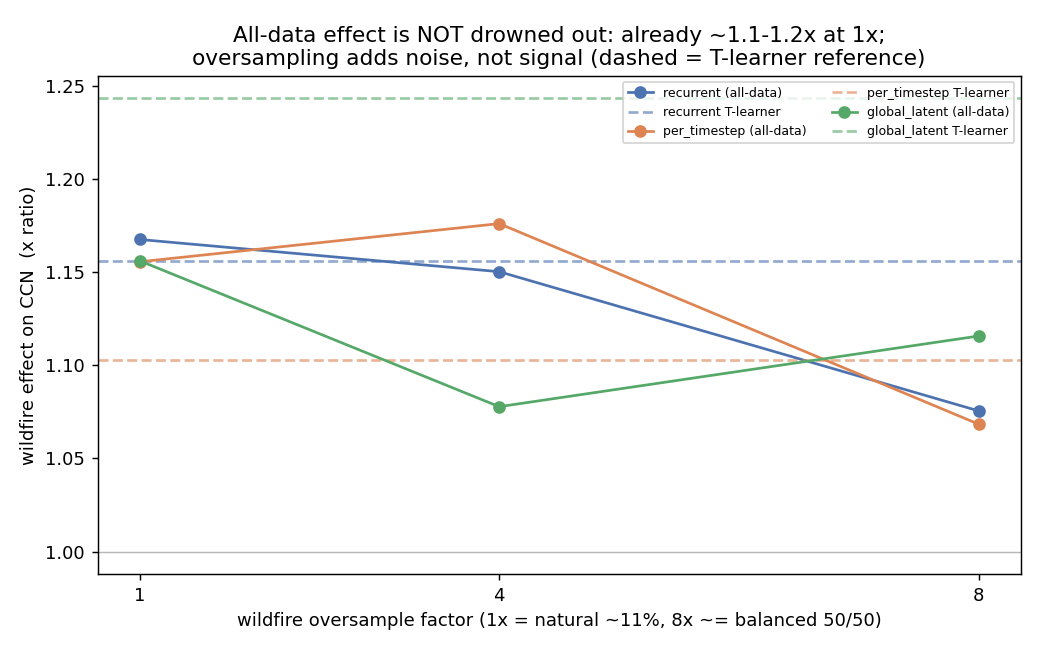
\includegraphics[width=0.80\textwidth]{attenuation_curve.png}
\caption{Effect from the all-data model (solid) vs.\ the two-model method (dashed),
for three model types. They agree, and giving the wildfire data more weight (left to
right) does not move the answer.}
\label{fig:agree}
\end{figure}

\section*{The three model types}
All three make the LSTM output a \emph{range} of possible CCN values (rather than a
single guess) by injecting Gaussian noise; they differ in where the noise enters and
how it varies across the trajectory:
\begin{itemize}
\item \textbf{Per-timestep}: a standard LSTM with a random noise vector concatenated
onto the weather inputs, redrawn \emph{fresh and independent at every timestep}.
\item \textbf{Global-latent}: the \emph{same} setup, except the noise vector is drawn
\emph{once per trajectory} and held fixed across all timesteps (one shared ``latent
code'').
\item \textbf{Recurrent}: unlike the other two, the noise is \emph{added to} the
LSTM's \emph{hidden state} (not concatenated to the inputs) at each step, so the
randomness \emph{accumulates} through the sequence.
\end{itemize}

\section*{Why the simpler model might work here (a hypothesis)}
We are \textbf{not sure} why the all-data model isn't swamped by the clean majority
($\sim$89\% of the data). One \emph{plausible} explanation: wildfire and clean periods
tend to occur in \emph{different weather}, so the model may be able to tell them apart
and lean on the wildfire examples at wildfire-weather rather than averaging everything
together --- which would also explain why adding weight to the wildfire data changed
little. We have not verified this mechanism; it is a hypothesis consistent with the
results, not a demonstrated cause.

\section*{What to keep in mind}
The small differences across settings are within noise (no error bars yet). If the
weather-separation explanation above is right, the simpler model would be a good
default only where that separation holds; if wildfire and clean conditions overlapped
more, it could start blending them.

\section*{Bottom line}
Both methods agree: wildfire adds roughly \textbf{15--20\% more CCN}, and the simpler
all-data model is enough for this dataset.

\end{document}
